\documentclass[11pt, oneside]{amsart}   	% use "amsart" instead of "article" for AMSLaTeX format
\usepackage{geometry}                		% See geometry.pdf to learn the layout options. There are lots.
\geometry{letterpaper}                   		% ... or a4paper or a5paper or ... 
%\geometry{landscape}                		% Activate for for rotated page geometry
%\usepackage[parfill]{parskip}    		% Activate to begin paragraphs with an empty line rather than an indent
\usepackage{graphicx}				% Use pdf, png, jpg, or eps� with pdflatex; use eps in DVI mode
								% TeX will automatically convert eps --> pdf in pdflatex		
\usepackage{amssymb}
\usepackage{listings}

\title{CS 325: Project 1}
\author{Group 29: Jacob Mastel, Yash Naik, Cera Olson}
\date{26 April 2015}							% Activate to display a given date or no date

\begin{document}
\maketitle
\newpage{}
\begin{figure}
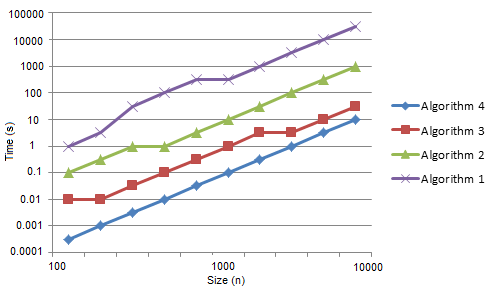
\includegraphics{AvgRunTime.png} [H]
\caption{Average Run Time for All 4 Algorithms}
\end{figure}

\section{Algorithm 1: Enumeration}
\subsection{Theoretical Run-Time Analysis}

Enumeration has a running time of $O(n^{3})$. Because of the 3 loops, each run n times gives the algorithm a running time of ${n*n*n}$.

\subsubsection{Pseudocode}
\begin{verbatim}
for i = 1 to n
	for j = i to n
		for k = i to j
			sum += a_k
		if  sum > ans then ans = sum
return ans
\end{verbatim}
	
\subsection{Experimental Analysis}
\begin{figure}
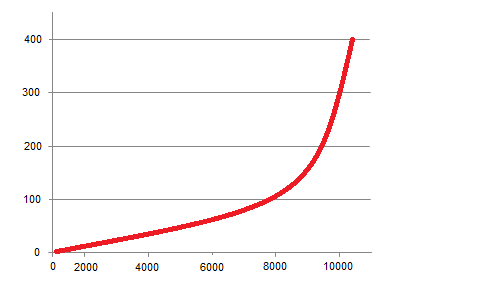
\includegraphics{Alg1Log.png}[H]
\caption{Algorithm 1 Run Time}
\end{figure}

\begin{center}
\begin{tabular}{ |c|c| } 
 \hline
 n & Time \\ 
100	& 0.029255198\\
200	& 0.178765495\\
300	& 0.541698859\\
400	& 1.337829466\\
500	& 2.473190885\\
600	& 4.287970855\\
700	& 7.054050103\\
800	& 10.06102867\\
900	& 15.23538047\\
1000	 & 20.64124558\\
1100	 & 26.77310262\\
1200	 & 31.31654893\\
1300	 & 39.63601268\\
1400	 & 49.22060823\\
1500	 & 60.55456953\\
1600	 & 73.94340321\\
1700	 & 84.80297324\\
1800	 & 99.51908661\\
1900	 & 117.1002546\\
2000	 & 136.9574863\\
 \hline
\end{tabular}
\end{center}

\subsection{Extrapolation and Interpretation}

\subsubsection{For each algorithm use the experimental data to estimate a function that models the relationship between running times and input sizes (n). Discuss any discrepancies between the experimental and theoretical running times.\\}

In an $O(n^3)$ algorithm, as n doubles the running times increases 8 fold. This means the running time increases significantly faster than the other versions of this algorithm. Right around n=9000, the algorithm begins to increase even faster than it was already. Of the 4 algorithms, it has the worst efficiency, and the experimental data supports that.  

\subsubsection{For each algorithm, what is the size of the biggest instance that you can solve with your algorithm in one hour?\\} 

When n doubles, the running time increases eightfold for an $O(n^3)$ algorithm. In one hour this algorithm can run approximately 4,000 values. $(1,000 *2^2)$.


\section{Algorithm 2: Better Enumeration}
\subsection{Theoretical Run-Time Analysis}

Because of the reduced number of loops, 2 loops running n times, the running time id $O(n^2)$. This algorithm runs very similarly to the first Algorithm, but it instead skips recalculating the sum each time through. This saves time and makes for a more efficient running time. 

\subsubsection{Pseudocode}
\begin{verbatim}
for i = 1 to n
	for j = i to n
		sum += a_j
	if  sum > ans then ans = sum
return ans
\end{verbatim}

\subsection{Experimental Analysis}
\begin{figure}
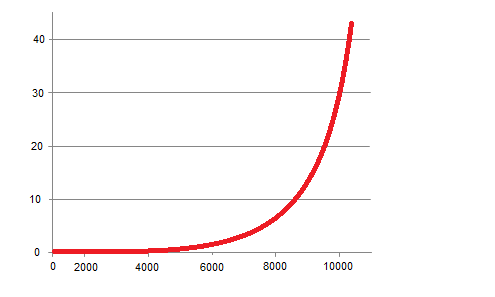
\includegraphics{Alg2Log.png}[H]
\caption{Algorithm 2 Run Time}
\end{figure}

\begin{center}
\begin{tabular}{ |c|c| } 
 \hline
 n & Time \\ 
100	& 0.000691457\\
200	& 0.002523139\\
300	& 0.005414918\\
400	& 0.009347594\\
500	& 0.017913874\\
600	& 0.032127009\\
700	& 0.03163984\\
800	& 0.037066278\\
900	& 0.076525134\\
1000 & 0.058382396\\
2000	 & 0.277541148\\
3000	 & 0.756019462\\
4000	 & 1.17740895\\
5000	 & 1.81821447\\
6000	 & 2.809200957\\
7000	 & 3.774356505\\
8000	 & 4.120086395\\
9000	 & 5.538109223\\
10000 & 6.983674863\\
20000 & 28.4940567\\
30000 & 67.27082063\\
 \hline
\end{tabular}
\end{center}

\subsection{Extrapolation and Interpretation}
\subsubsection{For each algorithm use the experimental data to estimate a function that models the relationship between running times and input sizes (n). Discuss any discrepancies between the experimental and theoretical running times.\\}

Using what we know about the algorithm and the experimental data, the data above supports the running time of $O(n^2)$. If you walk through the data, the running times increase by approximately a factor of 4. 

\subsubsection{For each algorithm, what is the size of the biggest instance that you can solve with your algorithm in one hour?\\}

When n doubles, the running time increases fourfold for an $O(n^2)$ algorithm. In one hour this algorithm can run approximately 320,000 values. $(10,000 *2^5)$.

\section{Algorithm 3: Divide and Conquer}

\subsection{Theoretical Run-Time Analysis}

The original problem size is a power of 2, so all sub sizes are integers. So the run time method of the program will be $O(n lg n)$. 
$T(n)=2T(n/2)+O(n)$ 

\subsubsection{Psuedocode}
\lstinputlisting[language=Python]{algorithm3.py}

\subsection{Proof of Correctness}

MaxSubarray(A, n) will return the sum of the maximum subarray of an array A of size n.

Proof: 
Base Case:- If n = 0. Then max = current = 0. Then subarray won�t be possible and the max will be zero for array of zero elements.
Case n=1: If n=1 meaning that there is one single element then if the value is positive it will be considered as array and max value will be assigned with the value of the array element.
Inductive hypothesis:-  Considering array contain more elements say �n�.
The method will find the sum of the whole array and save it in a variable max. and then it will divide the array in such a way that all the possible combinations of the array will be find and computed such that every loop execution the sum is compared with the max value if sum is greater then the value will be stored.
So while n>1 (meaning that more than one element in the array) the array will recursively divided and computes sum for all possible subarrays and compares with the max which will ultimately considered as the maximum value of a subarray.

\subsection{Experimental Analysis}
\begin{figure}
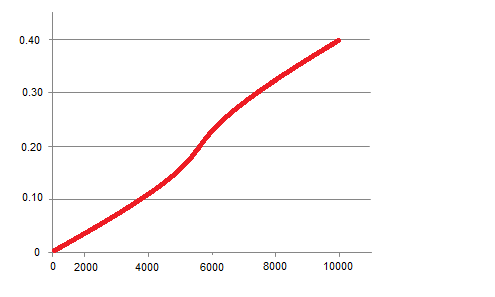
\includegraphics{Alg3Log.png}[H]
\caption{Algorithm 3 Run Time}
\end{figure}

\begin{center}
\begin{tabular}{ |c|c| } 
 \hline
 n & Time \\ 
100	& 0.000513281\\
1000	 & 0.004811525\\
2000 & 0.010599179\\
3000	 & 0.015096591\\
4000	 & 0.020326933\\
5000	 & 0.041936171\\
6000	 & 0.039872297\\
7000	 & 0.047068976\\
8000	 & 0.042948396\\
9000	 & 0.050002995\\
10000 & 0.054033207\\
20000 & 0.127373954\\
30000 & 0.194761927\\
40000 & 0.254894853\\
50000 & 0.31652922\\
60000 & 0.411895206\\
70000 & 0.450825678\\
80000 & 0.538815784\\
90000 & 0.589621596\\
100000 & 0.64801116\\
 \hline
\end{tabular}
\end{center}

\subsection{Extrapolation and Interpretation}
\subsubsection{For each algorithm use the experimental data to estimate a function that models the relationship between running times and input sizes (n). Discuss any discrepancies between the experimental and theoretical running times.\\}

While this graph was a bit less obvious, the general shape indicates a relationship similar to that of the linear running time. The data supports the theoretical running time of O(n log n) but just more than doubling each time n doubles. 

\subsubsection{For each algorithm, what is the size of the biggest instance that you can solve with your algorithm in one hour?\\}

When n doubles, the running time slightly more than doubles for an $O(n log n)$ algorithm. In one hour this algorithm can run approximately 409,600,000 values. $(100,000 *2^12)$.

\section{Algorithm 4: Linear-Time}
\subsection{Theoretical Run-Time Analysis}

Because there is only 1 loop that runs through n times the Linear Time Algorithm runs the fastest with a $O(n)$ running time. 

\subsubsection{Pseudocode}
\begin{verbatim}
for j = 1 .. n
	b = max{b + j, j}
    	ans = max{b, ans}
return ans
\end{verbatim}

\subsection{Experimental Analysis}
\begin{figure}
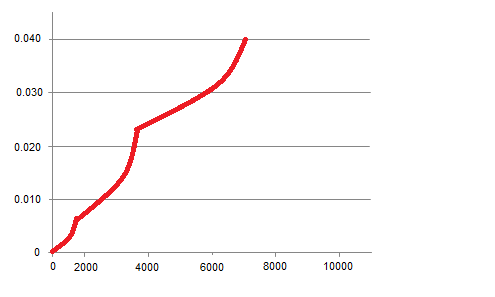
\includegraphics{Alg4Log.png}[H]
\caption{Algorithm 4 Run Time}
\end{figure}

\begin{center}
\begin{tabular}{ |c|c| } 
 \hline
 n & Time \\ 
100 & 0.00014592\\
1000	 & 0.000610561\\
2000	 & 0.001227777\\
3000	 & 0.00182733\\
4000	 & 0.002412802\\
5000	 & 0.002993667\\
6000	 & 0.003615748\\
7000	 & 0.004194308\\
8000	 & 0.004854277\\
9000	 & 0.005397254\\
10000 & 0.005966598\\
20000 & 0.011977484\\
30000 & 0.018128915\\
40000 & 0.034239523\\
50000 & 0.043462445\\
60000 & 0.037134118\\
70000 & 0.041755435\\
80000 & 0.061413183\\
90000 & 0.053687095\\
100000 & 0.061596479\\
 \hline
\end{tabular}
\end{center}

\subsection{Extrapolation and Interpretation}
\subsubsection{For each algorithm use the experimental data to estimate a function that models the relationship between running times and input sizes (n). Discuss any discrepancies between the experimental and theoretical running times.\\}

While the long term graph is a bit rough, the data supports a linear running time. Tracing through the data, the values follow the trend of doubling as n double. The exact data follows this trend in the long run, despite the few bumps.

\subsubsection{For each algorithm, what is the size of the biggest instance that you can solve with your algorithm in one hour?\\}

When n doubles, the running time doubles for an $O(n)$ algorithm. In one hour this algorithm can run approximately 3,276,800,000 values. $(100,000 *2^15)$.

\newpage{}
\section{Appendices}
\subsection{Code}
\subsubsection{Algorithm 1}
\lstinputlisting[language=Python]{algorithm1.py}
\subsubsection{Algorithm 2}
\lstinputlisting[language=Python]{algorithm2.py}
\subsubsection{Algorithm 3}
\lstinputlisting[language=Python]{algorithm3.py}
\subsubsection{Algorithm 4}
\lstinputlisting[language=Python]{algorithm4.py}

\subsection{Tests}
\lstinputlisting[language=Python]{main.py}		

\end{document}  